%**************************************%
%* Generated from MathBook XML source *%
%*    on 2016-11-06T22:27:34-05:00    *%
%*                                    *%
%*   http://mathbook.pugetsound.edu   *%
%*                                    *%
%**************************************%
\documentclass[10pt,]{book}
%% Custom Preamble Entries, early (use latex.preamble.early)
%% Inline math delimiters, \(, \), need to be robust
%% 2016-01-31:  latexrelease.sty  supersedes  fixltx2e.sty
%% If  latexrelease.sty  exists, bugfix is in kernel
%% If not, bugfix is in  fixltx2e.sty
%% See:  https://tug.org/TUGboat/tb36-3/tb114ltnews22.pdf
%% and read "Fewer fragile commands" in distribution's  latexchanges.pdf
\IfFileExists{latexrelease.sty}{}{\usepackage{fixltx2e}}
%% Text height identically 9 inches, text width varies on point size
%% See Bringhurst 2.1.1 on measure for recommendations
%% 75 characters per line (count spaces, punctuation) is target
%% which is the upper limit of Bringhurst's recommendations
%% Load geometry package to allow page margin adjustments
\usepackage{geometry}
\geometry{letterpaper,total={340pt,9.0in}}
%% Custom Page Layout Adjustments (use latex.geometry)
%% This LaTeX file may be compiled with pdflatex, xelatex, or lualatex
%% The following provides engine-specific capabilities
%% Generally, xelatex and lualatex will do better languages other than US English
%% You can pick from the conditional if you will only ever use one engine
\usepackage{ifthen}
\usepackage{ifxetex,ifluatex}
\ifthenelse{\boolean{xetex} \or \boolean{luatex}}{%
%% begin: xelatex and lualatex-specific configuration
%% fontspec package will make Latin Modern (lmodern) the default font
\ifxetex\usepackage{xltxtra}\fi
\usepackage{fontspec}
%% realscripts is the only part of xltxtra relevant to lualatex 
\ifluatex\usepackage{realscripts}\fi
%% 
%% Extensive support for other languages
\usepackage{polyglossia}
\setdefaultlanguage{english}
%% Magyar (Hungarian)
\setotherlanguage{magyar}
%% Spanish
\setotherlanguage{spanish}
%% Vietnamese
\setotherlanguage{vietnamese}
%% end: xelatex and lualatex-specific configuration
}{%
%% begin: pdflatex-specific configuration
%% translate common Unicode to their LaTeX equivalents
%% Also, fontenc with T1 makes CM-Super the default font
%% (\input{ix-utf8enc.dfu} from the "inputenx" package is possible addition (broken?)
\usepackage[T1]{fontenc}
\usepackage[utf8]{inputenc}
%% end: pdflatex-specific configuration
}
%% Monospace font: Inconsolata (zi4)
%% Sponsored by TUG: http://levien.com/type/myfonts/inconsolata.html
%% See package documentation for excellent instructions
%% One caveat, seem to need full file name to locate OTF files
%% Loads the "upquote" package as needed, so we don't have to
%% Upright quotes might come from the  textcomp  package, which we also use
%% We employ the shapely \ell to match Google Font version
%% pdflatex: "varqu" option produces best upright quotes
%% xelatex,lualatex: add StylisticSet 1 for shapely \ell
%% xelatex,lualatex: add StylisticSet 2 for plain zero
%% xelatex,lualatex: we add StylisticSet 3 for upright quotes
%% 
\ifthenelse{\boolean{xetex} \or \boolean{luatex}}{%
%% begin: xelatex and lualatex-specific monospace font
\usepackage{zi4}
\setmonofont[BoldFont=Inconsolatazi4-Bold.otf,StylisticSet={1,3}]{Inconsolatazi4-Regular.otf}
%% end: xelatex and lualatex-specific monospace font
}{%
%% begin: pdflatex-specific monospace font
\usepackage[varqu]{zi4}
%% end: pdflatex-specific monospace font
}
%% Symbols, align environment, bracket-matrix
\usepackage{amsmath}
\usepackage{amssymb}
%% allow more columns to a matrix
%% can make this even bigger by overriding with  latex.preamble.late  processing option
\setcounter{MaxMatrixCols}{30}
%%
%% Color support, xcolor package
%% Always loaded.  Used for:
%% mdframed boxes, add/delete text, author tools
\PassOptionsToPackage{usenames,dvipsnames,svgnames,table}{xcolor}
\usepackage{xcolor}
%%
%% Semantic Macros
%% To preserve meaning in a LaTeX file
%% Only defined here if required in this document
%% Used for inline definitions of terms
\newcommand{\terminology}[1]{\textbf{#1}}
%% Subdivision Numbering, Chapters, Sections, Subsections, etc
%% Subdivision numbers may be turned off at some level ("depth")
%% A section *always* has depth 1, contrary to us counting from the document root
%% The latex default is 3.  If a larger number is present here, then
%% removing this command may make some cross-references ambiguous
%% The precursor variable $numbering-maxlevel is checked for consistency in the common XSL file
\setcounter{secnumdepth}{3}
%% Environments with amsthm package
%% Theorem-like environments in "plain" style, with or without proof
\usepackage{amsthm}
\theoremstyle{plain}
%% Numbering for Theorems, Conjectures, Examples, Figures, etc
%% Controlled by  numbering.theorems.level  processing parameter
%% Always need a theorem environment to set base numbering scheme
%% even if document has no theorems (but has other environments)
\newtheorem{theorem}{Theorem}[section]
%% Only variants actually used in document appear here
%% Style is like a theorem, and for statements without proofs
%% Numbering: all theorem-like numbered consecutively
%% i.e. Corollary 4.3 follows Theorem 4.2
%% Definition-like environments, normal text
%% Numbering is in sync with theorems, etc
\theoremstyle{definition}
\newtheorem{definition}[theorem]{Definition}
%% Example-like environments, normal text
%% Numbering is in sync with theorems, etc
\theoremstyle{definition}
\newtheorem{example}[theorem]{Example}
%% Localize LaTeX supplied names (possibly none)
\renewcommand*{\appendixname}{Appendix}
\renewcommand*{\chaptername}{Chapter}
%% Equation Numbering
%% Controlled by  numbering.equations.level  processing parameter
\numberwithin{equation}{section}
%% Figures, Tables, Listings, Floats
%% The [H]ere option of the float package fixes floats in-place,
%% in deference to web usage, where floats are totally irrelevant
%% We re/define the figure, table and listing environments, if used
%%   1) New mbxfigure and/or mbxtable environments are defined with float package
%%   2) Standard LaTeX environments redefined to use new environments
%%   3) Standard LaTeX environments redefined to step theorem counter
%%   4) Counter for new environments is set to the theorem counter before caption
%% You can remove all this figure/table setup, to restore standard LaTeX behavior
%% HOWEVER, numbering of figures/tables AND theorems/examples/remarks, etc
%% WILL ALL de-synchronize with the numbering in the HTML version
%% You can remove the [H] argument of the \newfloat command, to allow flotation and 
%% preserve numbering, BUT the numbering may then appear "out-of-order"
\usepackage{float}
\usepackage[bf]{caption} % http://tex.stackexchange.com/questions/95631/defining-a-new-type-of-floating-environment 
\usepackage{newfloat}
% Figure environment setup so that it no longer floats
\SetupFloatingEnvironment{figure}{fileext=lof,placement={H},within=section,name=Figure}
% figures have the same number as theorems: http://tex.stackexchange.com/questions/16195/how-to-make-equations-figures-and-theorems-use-the-same-numbering-scheme 
\makeatletter
\let\c@figure\c@theorem
\makeatother
%% Footnote Numbering
%% We reset the footnote counter, as given by numbering.footnotes.level
\makeatletter\@addtoreset{footnote}{section}\makeatother
%% Raster graphics inclusion, wrapped figures in paragraphs
%% \resizebox sometimes used for images in side-by-side layout
\usepackage{graphicx}
%%
%% Program listing support, for inline code, Sage code
\usepackage{listings}
%% We define the listings font style to be the default "ttfamily"
%% To fix hyphens/dashes rendered in PDF as fancy minus signs by listing
%% http://tex.stackexchange.com/questions/33185/listings-package-changes-hyphens-to-minus-signs
\makeatletter
\lst@CCPutMacro\lst@ProcessOther {"2D}{\lst@ttfamily{-{}}{-{}}}
\@empty\z@\@empty
\makeatother
\ifthenelse{\boolean{xetex}}{}{%
%% begin: pdflatex-specific listings configuration
%% translate U+0080 - U+00F0 to their textmode LaTeX equivalents
%% Data originally from https://www.w3.org/Math/characters/unicode.xml, 2016-07-23
%% Lines marked in XSL with "$" were converted from mathmode to textmode
\lstset{extendedchars=true}
\lstset{literate={ }{{~}}{1}{¡}{{\textexclamdown }}{1}{¢}{{\textcent }}{1}{£}{{\textsterling }}{1}{¤}{{\textcurrency }}{1}{¥}{{\textyen }}{1}{¦}{{\textbrokenbar }}{1}{§}{{\textsection }}{1}{¨}{{\textasciidieresis }}{1}{©}{{\textcopyright }}{1}{ª}{{\textordfeminine }}{1}{«}{{\guillemotleft }}{1}{¬}{{\textlnot }}{1}{­}{{\-}}{1}{®}{{\textregistered }}{1}{¯}{{\textasciimacron }}{1}{°}{{\textdegree }}{1}{±}{{\textpm }}{1}{²}{{\texttwosuperior }}{1}{³}{{\textthreesuperior }}{1}{´}{{\textasciiacute }}{1}{µ}{{\textmu }}{1}{¶}{{\textparagraph }}{1}{·}{{\textperiodcentered }}{1}{¸}{{\c{}}}{1}{¹}{{\textonesuperior }}{1}{º}{{\textordmasculine }}{1}{»}{{\guillemotright }}{1}{¼}{{\textonequarter }}{1}{½}{{\textonehalf }}{1}{¾}{{\textthreequarters }}{1}{¿}{{\textquestiondown }}{1}{À}{{\`{A}}}{1}{Á}{{\'{A}}}{1}{Â}{{\^{A}}}{1}{Ã}{{\~{A}}}{1}{Ä}{{\"{A}}}{1}{Å}{{\AA }}{1}{Æ}{{\AE }}{1}{Ç}{{\c{C}}}{1}{È}{{\`{E}}}{1}{É}{{\'{E}}}{1}{Ê}{{\^{E}}}{1}{Ë}{{\"{E}}}{1}{Ì}{{\`{I}}}{1}{Í}{{\'{I}}}{1}{Î}{{\^{I}}}{1}{Ï}{{\"{I}}}{1}{Ð}{{\DH }}{1}{Ñ}{{\~{N}}}{1}{Ò}{{\`{O}}}{1}{Ó}{{\'{O}}}{1}{Ô}{{\^{O}}}{1}{Õ}{{\~{O}}}{1}{Ö}{{\"{O}}}{1}{×}{{\texttimes }}{1}{Ø}{{\O }}{1}{Ù}{{\`{U}}}{1}{Ú}{{\'{U}}}{1}{Û}{{\^{U}}}{1}{Ü}{{\"{U}}}{1}{Ý}{{\'{Y}}}{1}{Þ}{{\TH }}{1}{ß}{{\ss }}{1}{à}{{\`{a}}}{1}{á}{{\'{a}}}{1}{â}{{\^{a}}}{1}{ã}{{\~{a}}}{1}{ä}{{\"{a}}}{1}{å}{{\aa }}{1}{æ}{{\ae }}{1}{ç}{{\c{c}}}{1}{è}{{\`{e}}}{1}{é}{{\'{e}}}{1}{ê}{{\^{e}}}{1}{ë}{{\"{e}}}{1}{ì}{{\`{\i}}}{1}{í}{{\'{\i}}}{1}{î}{{\^{\i}}}{1}{ï}{{\"{\i}}}{1}{ð}{{\dh }}{1}{ñ}{{\~{n}}}{1}{ò}{{\`{o}}}{1}{ó}{{\'{o}}}{1}{ô}{{\^{o}}}{1}{õ}{{\~{o}}}{1}{ö}{{\"{o}}}{1}{÷}{{\textdiv }}{1}{ø}{{\o }}{1}{ù}{{\`{u}}}{1}{ú}{{\'{u}}}{1}{û}{{\^{u}}}{1}{ü}{{\"{u}}}{1}{ý}{{\'{y}}}{1}{þ}{{\th }}{1}{ÿ}{{\"{y}}}{1}}
%% end: pdflatex-specific listings configuration
}
%% End of generic listing adjustments
%% Sage's blue is 50%, we go way lighter (blue!05 would work)
\definecolor{sageblue}{rgb}{0.95,0.95,1}
%% Sage input, listings package: Python syntax, boxed, colored, line breaking
%% Indent from left margin, flush at right margin
\lstdefinestyle{sageinput}{language=Python,breaklines=true,breakatwhitespace=true,basicstyle=\small\ttfamily,columns=fixed,frame=single,backgroundcolor=\color{sageblue},xleftmargin=4ex}
%% Sage output, similar, but not boxed, not colored
\lstdefinestyle{sageoutput}{language=Python,breaklines=true,breakatwhitespace=true,basicstyle=\small\ttfamily,columns=fixed,xleftmargin=4ex}
%% More flexible list management, esp. for references and exercises
%% But also for specifying labels (i.e. custom order) on nested lists
\usepackage{enumitem}
%% Support for index creation
%% imakeidx package does not require extra pass (as with makeidx)
%% We set the title of the "Index" section via a keyword
%% And we provide language support for the "see" phrase
\usepackage{imakeidx}
\makeindex[title=Index, intoc=true]
\renewcommand{\seename}{see}
%% hyperref driver does not need to be specified
\usepackage{hyperref}
%% configure hyperref's  \url  to match listings' inline verbatim
\renewcommand\UrlFont{\small\ttfamily}
%% Hyperlinking active in PDFs, all links solid and blue
\hypersetup{colorlinks=true,linkcolor=blue,citecolor=blue,filecolor=blue,urlcolor=blue}
\hypersetup{pdftitle={Differential Equations Lecture Notes for Fall 2016}}
%% If you manually remove hyperref, leave in this next command
\providecommand\phantomsection{}
%% If tikz has been loaded, replace ampersand with \amp macro
%% extpfeil package for certain extensible arrows,
%% as also provided by MathJax extension of the same name
%% NB: this package loads mtools, which loads calc, which redefines
%%     \setlength, so it can be removed if it seems to be in the 
%%     way and your math does not use:
%%     
%%     \xtwoheadrightarrow, \xtwoheadleftarrow, \xmapsto, \xlongequal, \xtofrom
%%     
%%     we have had to be extra careful with variable thickness
%%     lines in tables, and so also load this package late
\usepackage{extpfeil}
%% Custom Preamble Entries, late (use latex.preamble.late)
%% Begin: Author-provided packages
%% (From  docinfo/latex-preamble/package  elements)
%% End: Author-provided packages
%% Begin: Author-provided macros
%% (From  docinfo/macros  element)
%% Plus three from MBX for XML characters

\newcommand{\lt}{ < }
\newcommand{\gt}{ > }
\newcommand{\amp}{ & }
%% End: Author-provided macros
%% Title page information for book
\title{Differential Equations Lecture Notes for Fall 2016\\
{\large West Virginia Wesleyan College}}
\author{}
\date{}
\begin{document}
\typeout{************************************************}
\typeout{Chapter 1 Fourier Analysis}
\typeout{************************************************}
\chapter[{Fourier Analysis}]{Fourier Analysis}\label{fourier-analysis}
\typeout{************************************************}
\typeout{Introduction  }
\typeout{************************************************}
Our goal now is to move to solving \emph{partial} differential equations (PDEs), which are differential equations that involve multiple independent variables. Such equations are particularly useful for modeling quantities that depend on position \(x\) and time \(t\). It turns out that these partial differential equations often involve periodic functions. So our first step to solving PDEs will be to find useful descriptions of periodic (and in some cases, non-periodic) functions.%
\typeout{************************************************}
\typeout{Section 1.1 Fourier Series}
\typeout{************************************************}
\section[{Fourier Series}]{Fourier Series}\label{section-fourier-series}
The main idea behind Fourier series, and the field of harmonic analysis in general, is to represent more complicated objects in terms of simpler objects. A fundamental example of this idea comes from the field of linear algebra in the form of \emph{orthonormal bases}. Knowing an orthonormal basis for a vector space \(V\) can greatly simplify linear algebra in that vector space. In this section, we'll do something similar with periodic functions.%
\typeout{************************************************}
\typeout{Subsection 1.1.1 Periodic Functions}
\typeout{************************************************}
\subsection[{Periodic Functions}]{Periodic Functions}\label{subsection-periodic-functions}
Consider the function \(f(x)\) given by the following graph:%
\leavevmode%
\begin{figure}
\centering
\IfFileExists{images/image-sageplot-periodic-function.pdf}%
{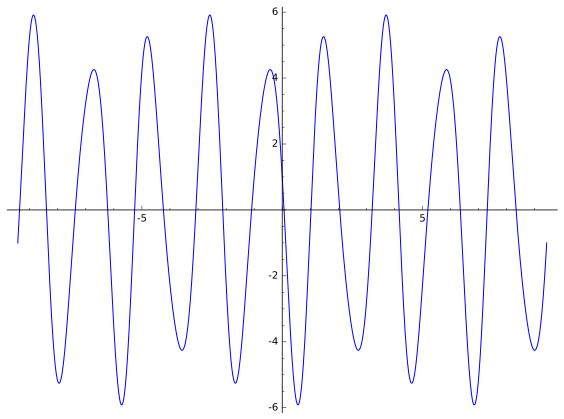
\includegraphics[width=1\linewidth]{images/image-sageplot-periodic-function.pdf}}%
% {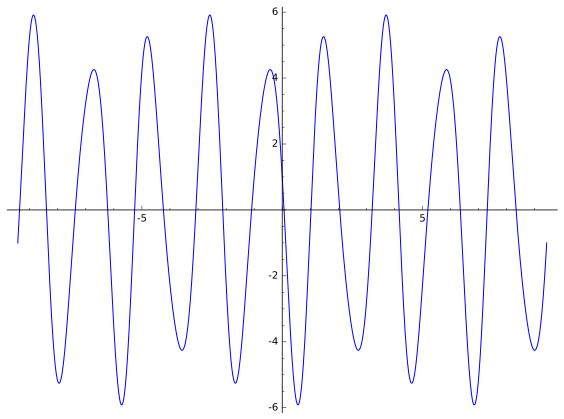
\includegraphics[width=1\linewidth]{images/image-sageplot-periodic-function.png}}
\caption{A periodic function.\label{figure-sageplot-periodic-function}}
\end{figure}
\par
This function can be plotted using the following code:%
\begin{lstlisting}[style=sageinput]
reset

import matplotlib.pyplot as plt
import numpy as np

# The following is here to adjust text on the graph... not a huge deal.
from matplotlib import rc
rc('font',**{'family':'sans-serif','sans-serif':['Helvetica']})
rc('text', usetex=True)

# This is setting up our graph.
x = np.linspace(-3*np.pi,3*np.pi,200)
y1 = np.cos(5*x)
y2 = np.sin(.5*x)

# This actually plots the graph.
p = plt.plot(x,y1-5*y2,label=r'$f(x)$')
plt.legend()
\end{lstlisting}
\par
If we look at the graph, we see that it repeats itself if we wait long enough. Functions that have this property are called \terminology{periodic functions}.%
\begin{definition}[{Periodic Functions}]\label{definition-periodic-functions}
\index{Functions!periodic}Let \(f(x)\) be a real function defined for all \(x\). We say that \(f\) is a periodic function if there exists a positive number \(p\) such that
                    \begin{equation*}
                        f(x+p) = f(x)
                    \end{equation*}
                    for all \(x\).%
\end{definition}

                
                Let \(n\) be any integer. Then the functions \(\sin nx\) and \(\cos nx\) are both periodic and have period \(2\pi\) since
                \begin{align*}
\sin[n(x+2\pi)] & = \sin nx\cos2\pi + \cos nx\sin2\pi = \sin nx \\
\cos[n(x+2\pi)] & = \cos nx\cos2\pi - \sin nx\sin2\pi = \cos nx 
\end{align*}
                The periodic nature of these functions can also be seen from their graphs:%

                \begin{lstlisting}[style=sageinput]
# This is setting up our graph.
x = np.linspace(-3*np.pi,3*np.pi,200)
y1 = np.cos(5*x)
y2 = np.sin(2*x)

# This actually plots the graphs.
plt.subplot(2,1,1)
plt.plot(x,y1,label=r'$\cos5x$')
plt.legend()

plt.subplot(2,1,2)
plt.plot(x,y2,label=r'$\sin2x$')
plt.legend()
plt.show()
\end{lstlisting}

            \par
If you go back to the first plot, you may notice from the code used to generate the function \(f(x)\) that \(f(x)\) is just the sum of two basic trigonometric functions:
            \begin{equation*}f(x) = \cos5x-5\sin\frac{x}{2}.\end{equation*}
            In other words, the (finite) sum of functions of the form \(\sin nx,\cos mx\) where \(n,m\) are real numbers is also periodic, and also has period \(2\pi\). One of the greatest accomplishments in mathematics was the realization that many other periodic functions can be written in this way, if we allow \emph{infinite} sums of this form, which we call \terminology{trigonometric series}.%
\typeout{************************************************}
\typeout{Subsection 1.1.2 Trigonometric Series and Fourier Series}
\typeout{************************************************}
\subsection[{Trigonometric Series and Fourier Series}]{Trigonometric Series and Fourier Series}\label{subsection-trig-and-fourier-series}
\begin{definition}[{Trigonometric Series}]\label{definition-trigonometric-series}
\index{Series!trigonometric}A trigonometric series is a series of the form
                    \begin{equation*}\sum_{k=0}^{\infty}(a_{k}\cos kx+b_{k}\sin kx) = a_{0} + \sum_{k=1}^{\infty}(a_{k}\cos kx+b_{k}\sin kx)\end{equation*}
                    where \(a_{k},b_{k}\) are constants, called the \terminology{coefficients} of the series.%
\end{definition}
Our primary goal in this section is to take a function \(f(x)\) of period \(2\pi\) and express it as a trigonometric series. To see how, we'll suppose that we have the trigonometric series we want, i.e. that
            \begin{equation*}f(x) = a_{0} + \sum_{k=1}^{\infty}(a_{k}\cos kx+b_{k}\sin kx),\end{equation*}
            and we'll look at what the coefficients of the series need to be to make this equation true. To do this, we'll need the so-called \terminology{orthogonality relations} for \(\sin nx,\cos mx\)%
\begin{theorem}[{Orthogonality Relations}]\label{theorem-orthogonality-relations}
\index{Orthogonality relations}Let \(m,n\) be whole numbers with \(m,n>0\). Then
                    \begin{equation*}\int_{-\pi}^{\pi}\sin mx\cos nx\,dx = 0\end{equation*}
                    and
                    \begin{equation*}\int_{-\pi}^{\pi}\sin mx\sin nx\,dx = \begin{cases} \pi & m=n \\ 0 & m\neq n\end{cases}\text{ and }\int_{-\pi}^{\pi}\cos mx\cos nx\,dx = \begin{cases} \pi & m=n \\ 0 & m\neq n\end{cases}\end{equation*}%
\end{theorem}
\par
We can verify Theorem \hyperref[theorem-orthogonality-relations]{\ref{theorem-orthogonality-relations}} using a computer algebra system. Proving it is a little bit more work, but can be done using trigonometric identities or Euler's formula.%
\begin{lstlisting}[style=sageinput]
# Declare variables.
var('x,m,n')
assume(m,n,'integer')

# Perform the integrations.
I1 = integral(sin(m*x)*cos(n*x),x,-pi,pi)
I2 = integral(sin(m*x)*sin(n*x),x,-pi,pi)
I3 = integral(cos(m*x)*cos(n*x),x,-pi,pi)
I4 = integral(sin(m*x)*sin(m*x),x,-pi,pi)
I5 = integral(cos(n*x)*cos(n*x),x,-pi,pi)

# List the results.
I1,I2,I3,I4,I5
\end{lstlisting}
\par
Theorem \hyperref[theorem-orthogonality-relations]{\ref{theorem-orthogonality-relations}} will be our primary tool for expressing a function \(f(x)\) as a trigonometric series. To see how, suppose that we have
            \begin{equation*}f(x) = a_{0} + \sum_{k=1}^{\infty}(a_{k}\cos kx+b_{k}\sin kx).\end{equation*}
            If this equation were true, then we should be able to integrate both sides of it and get another true equation. Since Theorem \hyperref[theorem-orthogonality-relations]{\ref{theorem-orthogonality-relations}} suggests that integrals involving \(\sin nx,\cos nx\) simplify very nicely, we'll try to integrate both sides of the equation against \(\sin nx,\cos nx\) from \(x=-\pi\) to \(x=\pi\) for some \(n>0\). If we do this, we get
            \begin{align*}
\int_{-\pi}^{\pi}f(x)\sin nx\,dx & = a_{0}\int_{-\pi}^{\pi}\sin nx\,dx + \sum_{k=1}^{\infty}\left(a_{k}\int_{-\pi}^{\pi}\cos kx\sin nx\,dx + b_{k}\int_{-\pi}^{\pi}\sin kx\sin nx\,dx\right)\\
 & = b_{n}\int_{-\pi}^{\pi}\sin nx \sin nx \,dx\\
 & = \pi b_{n}
\end{align*}
            This lets us solve for \(b_{n}\)! We have
            \begin{equation*}b_{n} = \frac{1}{\pi}\int_{-\pi}^{\pi}f(x)\sin nx\,dx\text{ for $n\geq 1$.}\end{equation*}
            Similarly,
            \begin{align*}
a_{n} & = \frac{1}{\pi}\int_{-\pi}^{\pi}f(x)\cos nx\,dx\text{ for $n\geq1$.}\\
a_{0} & = \frac{1}{2\pi}\int_{-\pi}^{\pi}f(x)\,dx
\end{align*}
            %
\begin{example}[The Fourier series of \(x^{3}\)]\label{example-fourier-series-of-absolute-value}
Define \(f(x) = x^{3}\) for \(-\pi\leq x\leq \pi\). To find its Fourier series, we can just use the previous formulas to find the values of the coefficients \(a_{0},a_{k},b_{k}\) for \(k\geq1\). We know that
                \begin{align*}
a_{0} & = \frac{1}{2\pi}\int_{-\pi}^{\pi}x^{3}\,dx\\
a_{k} & = \frac{1}{\pi}\int_{-\pi}^{\pi}x^{3}\cos kx\,dx \\
b_{k} & = \frac{1}{\pi}\int_{-\pi}^{\pi}x^{3}\sin kx\,dx.
\end{align*}
                As nasty as these are, the first two are actually very easy to compute. Here's why: \(x^{3}\) and \(x^{3}\cos kx\) are both \emph{odd} functions, and the integral of any odd function in an interval that is symmetric about \(0\) is always \(0\) (since the areas cancel out). So \(a_{0} = a_{k} = 0\) for all \(k\geq0\). The last term is a bit more complicated, but we can use integration by parts (and I definitely recommend using a computer here) to show that
                \begin{equation*}
                    \int x^{3}\sin kx\,dx = -\frac{{\left(k^{3} x^{3} - 6 \, k x\right)} \cos\left(k x\right) - 3 \, {\left(k^{2} x^{2} - 2\right)} \sin\left(k x\right)}{k^{4}} + C.
                \end{equation*}
                If we plug in the limits of integration and simplify (again, computers are handy for this!), we get
                \begin{equation*}
                    b_{k} = \frac{2 \, {\left(6 \, \pi - \pi^{3} k^{2}\right)} \left(-1\right)^{k}}{\pi k^{3}}.
                \end{equation*}
                So the Fourier series for \(f(x) = x^{3}\) is given by
                \begin{align*}
a_{0} + \sum_{k=1}^{\infty}(a_{k}\cos kx+b_{k}\sin kx) &= \sum_{k=1}^{\infty}b_{k}\sin kx \\
 &= \sum_{k=1}^{\infty}\frac{2 \, {\left(6 \, \pi - \pi^{3} k^{2}\right)} \left(-1\right)^{k}}{\pi k^{3}}\sin kx. 
\end{align*}
                %
\end{example}
\par
A very good question at this point is, what relationship does the Fourier series that we found in the previous example have with the original function \(f(x)\)? Are they actually equal? If we use the following code (adapted from \href{https://doxdrum.wordpress.com/2011/01/31/sage-tip-fourier-series-approximation/}{here}) to compare the partial sums
            \begin{equation*}
                \sum_{k=1}^{n}\frac{2 \, {\left(6 \, \pi - \pi^{3} k^{2}\right)} \left(-1\right)^{k}}{\pi k^{3}}\sin kx
            \end{equation*}
            of the Fourier series with \(f(x) = x^{3}\), then it looks like the partial sums get closer and closer if we choose larger values of \(n\).%
\begin{lstlisting}[style=sageinput]
var('x,k,i')

# Defines the function to determine Fourier series of. Feel free to play around with this.
f(x) = x**3

# Defines the Fourier coefficients.
def a(k):
    coeff = integral(f(x)*cos(k*x), (x,-pi,pi))/pi
    return coeff

def b(k):
    coeff = integral(f(x)*sin(k*x), (x,-pi,pi))/pi
    return coeff

# Defines the corresponding (partial) Fourier series.
def FS(k): 
    return a(0)/2 + sum(a(i)*cos(i*x) + b(i)*sin(i*x), i, 1, k)

n = 3
p = plot(FS(n),(x,-pi,pi), color='red') + plot(f(x),(x,-pi,pi))
p
\end{lstlisting}
\par
In general, the question of whether or not a given Fourier series makes sense is a difficult one to answer.
However, for many of the functions we care about in this course we have the following theorem.%
\begin{theorem}[{Fourier Series of Piecewise Continuous Functions}]\label{theorem-pointwise-convergence-of-fourier-series}
\index{Fourier series!convergence}
                        Let \(f(x)\) be a piecewise continuous function on the interval \(-\pi\leq x\leq\pi\), and suppose that it's also periodic with period \(2\pi\), and is differentiable everywhere that it's continuous. Then the Fourier series of \(f(x)\) converges to \(f(x)\) except at the points where \(f(x)\) is continuous.
                    \end{theorem}
%
%% A lineskip in table of contents as transition to appendices, backmatter
\addtocontents{toc}{\vspace{\normalbaselineskip}}
%
%
\appendix
%
\typeout{************************************************}
\typeout{Appendix A GNU Free Documentation License}
\typeout{************************************************}
\chapter[{GNU Free Documentation License}]{GNU Free Documentation License}\label{appendix-gfdl}
\typeout{************************************************}
\typeout{Paragraphs  }
\typeout{************************************************}
\paragraph[{}]{}\hypertarget{paragraphs-1}{}
Version 1.3, 3 November 2008%
\par
Copyright \textcopyright{} 2000, 2001, 2002, 2007, 2008 Free Software Foundation, Inc. \textless{}\url{http://www.fsf.org/}\textgreater{}%
\par
Everyone is permitted to copy and distribute verbatim copies of this license document, but changing it is not allowed.%
\typeout{************************************************}
\typeout{Paragraphs  0. PREAMBLE}
\typeout{************************************************}
\paragraph[{0. PREAMBLE}]{0. PREAMBLE}\hypertarget{gfdl-section0}{}
The purpose of this License is to make a manual, textbook, or other functional and useful document ``free'' in the sense of freedom: to assure everyone the effective freedom to copy and redistribute it, with or without modifying it, either commercially or noncommercially. Secondarily, this License preserves for the author and publisher a way to get credit for their work, while not being considered responsible for modifications made by others.%
\par
This License is a kind of ``copyleft'', which means that derivative works of the document must themselves be free in the same sense. It complements the GNU General Public License, which is a copyleft license designed for free software.%
\par
We have designed this License in order to use it for manuals for free software, because free software needs free documentation: a free program should come with manuals providing the same freedoms that the software does. But this License is not limited to software manuals; it can be used for any textual work, regardless of subject matter or whether it is published as a printed book. We recommend this License principally for works whose purpose is instruction or reference.%
\typeout{************************************************}
\typeout{Paragraphs  1. APPLICABILITY AND DEFINITIONS}
\typeout{************************************************}
\paragraph[{1. APPLICABILITY AND DEFINITIONS}]{1. APPLICABILITY AND DEFINITIONS}\hypertarget{gfdl-section1}{}
This License applies to any manual or other work, in any medium, that contains a notice placed by the copyright holder saying it can be distributed under the terms of this License. Such a notice grants a world-wide, royalty-free license, unlimited in duration, to use that work under the conditions stated herein. The ``Document'', below, refers to any such manual or work. Any member of the public is a licensee, and is addressed as ``you''. You accept the license if you copy, modify or distribute the work in a way requiring permission under copyright law.%
\par
A ``Modified Version'' of the Document means any work containing the Document or a portion of it, either copied verbatim, or with modifications and/or translated into another language.%
\par
A ``Secondary Section'' is a named appendix or a front-matter section of the Document that deals exclusively with the relationship of the publishers or authors of the Document to the Document's overall subject (or to related matters) and contains nothing that could fall directly within that overall subject. (Thus, if the Document is in part a textbook of mathematics, a Secondary Section may not explain any mathematics.) The relationship could be a matter of historical connection with the subject or with related matters, or of legal, commercial, philosophical, ethical or political position regarding them.%
\par
The ``Invariant Sections'' are certain Secondary Sections whose titles are designated, as being those of Invariant Sections, in the notice that says that the Document is released under this License. If a section does not fit the above definition of Secondary then it is not allowed to be designated as Invariant. The Document may contain zero Invariant Sections. If the Document does not identify any Invariant Sections then there are none.%
\par
The ``Cover Texts'' are certain short passages of text that are listed, as Front-Cover Texts or Back-Cover Texts, in the notice that says that the Document is released under this License. A Front-Cover Text may be at most 5 words, and a Back-Cover Text may be at most 25 words.%
\par
A ``Transparent'' copy of the Document means a machine-readable copy, represented in a format whose specification is available to the general public, that is suitable for revising the document straightforwardly with generic text editors or (for images composed of pixels) generic paint programs or (for drawings) some widely available drawing editor, and that is suitable for input to text formatters or for automatic translation to a variety of formats suitable for input to text formatters. A copy made in an otherwise Transparent file format whose markup, or absence of markup, has been arranged to thwart or discourage subsequent modification by readers is not Transparent. An image format is not Transparent if used for any substantial amount of text. A copy that is not ``Transparent'' is called ``Opaque''.%
\par
Examples of suitable formats for Transparent copies include plain ASCII without markup, Texinfo input format, LaTeX input format, SGML or XML using a publicly available DTD, and standard-conforming simple HTML, PostScript or PDF designed for human modification. Examples of transparent image formats include PNG, XCF and JPG. Opaque formats include proprietary formats that can be read and edited only by proprietary word processors, SGML or XML for which the DTD and/or processing tools are not generally available, and the machine-generated HTML, PostScript or PDF produced by some word processors for output purposes only.%
\par
The ``Title Page'' means, for a printed book, the title page itself, plus such following pages as are needed to hold, legibly, the material this License requires to appear in the title page. For works in formats which do not have any title page as such, ``Title Page'' means the text near the most prominent appearance of the work's title, preceding the beginning of the body of the text.%
\par
The ``publisher'' means any person or entity that distributes copies of the Document to the public.%
\par
A section ``Entitled XYZ'' means a named subunit of the Document whose title either is precisely XYZ or contains XYZ in parentheses following text that translates XYZ in another language. (Here XYZ stands for a specific section name mentioned below, such as ``Acknowledgements'', ``Dedications'', ``Endorsements'', or ``History''.) To ``Preserve the Title'' of such a section when you modify the Document means that it remains a section ``Entitled XYZ'' according to this definition.%
\par
The Document may include Warranty Disclaimers next to the notice which states that this License applies to the Document. These Warranty Disclaimers are considered to be included by reference in this License, but only as regards disclaiming warranties: any other implication that these Warranty Disclaimers may have is void and has no effect on the meaning of this License.%
\typeout{************************************************}
\typeout{Paragraphs  2. VERBATIM COPYING}
\typeout{************************************************}
\paragraph[{2. VERBATIM COPYING}]{2. VERBATIM COPYING}\hypertarget{gfdl-section2}{}
You may copy and distribute the Document in any medium, either commercially or noncommercially, provided that this License, the copyright notices, and the license notice saying this License applies to the Document are reproduced in all copies, and that you add no other conditions whatsoever to those of this License. You may not use technical measures to obstruct or control the reading or further copying of the copies you make or distribute. However, you may accept compensation in exchange for copies. If you distribute a large enough number of copies you must also follow the conditions in section 3.%
\par
You may also lend copies, under the same conditions stated above, and you may publicly display copies.%
\typeout{************************************************}
\typeout{Paragraphs  3. COPYING IN QUANTITY}
\typeout{************************************************}
\paragraph[{3. COPYING IN QUANTITY}]{3. COPYING IN QUANTITY}\hypertarget{gfdl-section3}{}
If you publish printed copies (or copies in media that commonly have printed covers) of the Document, numbering more than 100, and the Document's license notice requires Cover Texts, you must enclose the copies in covers that carry, clearly and legibly, all these Cover Texts: Front-Cover Texts on the front cover, and Back-Cover Texts on the back cover. Both covers must also clearly and legibly identify you as the publisher of these copies. The front cover must present the full title with all words of the title equally prominent and visible. You may add other material on the covers in addition. Copying with changes limited to the covers, as long as they preserve the title of the Document and satisfy these conditions, can be treated as verbatim copying in other respects.%
\par
If the required texts for either cover are too voluminous to fit legibly, you should put the first ones listed (as many as fit reasonably) on the actual cover, and continue the rest onto adjacent pages.%
\par
If you publish or distribute Opaque copies of the Document numbering more than 100, you must either include a machine-readable Transparent copy along with each Opaque copy, or state in or with each Opaque copy a computer-network location from which the general network-using public has access to download using public-standard network protocols a complete Transparent copy of the Document, free of added material. If you use the latter option, you must take reasonably prudent steps, when you begin distribution of Opaque copies in quantity, to ensure that this Transparent copy will remain thus accessible at the stated location until at least one year after the last time you distribute an Opaque copy (directly or through your agents or retailers) of that edition to the public.%
\par
It is requested, but not required, that you contact the authors of the Document well before redistributing any large number of copies, to give them a chance to provide you with an updated version of the Document.%
\typeout{************************************************}
\typeout{Paragraphs  4. MODIFICATIONS}
\typeout{************************************************}
\paragraph[{4. MODIFICATIONS}]{4. MODIFICATIONS}\hypertarget{gfdl-section4}{}
You may copy and distribute a Modified Version of the Document under the conditions of sections 2 and 3 above, provided that you release the Modified Version under precisely this License, with the Modified Version filling the role of the Document, thus licensing distribution and modification of the Modified Version to whoever possesses a copy of it. In addition, you must do these things in the Modified Version:%
\leavevmode%
\begin{enumerate}[label=\Alph*.]
\item\hypertarget{li-1}{}Use in the Title Page (and on the covers, if any) a title distinct from that of the Document, and from those of previous versions (which should, if there were any, be listed in the History section of the Document). You may use the same title as a previous version if the original publisher of that version gives permission.%
\item\hypertarget{li-2}{}List on the Title Page, as authors, one or more persons or entities responsible for authorship of the modifications in the Modified Version, together with at least five of the principal authors of the Document (all of its principal authors, if it has fewer than five), unless they release you from this requirement.%
\item\hypertarget{li-3}{}State on the Title page the name of the publisher of the Modified Version, as the publisher.%
\item\hypertarget{li-4}{}Preserve all the copyright notices of the Document.%
\item\hypertarget{li-5}{}Add an appropriate copyright notice for your modifications adjacent to the other copyright notices.%
\item\hypertarget{li-6}{}Include, immediately after the copyright notices, a license notice giving the public permission to use the Modified Version under the terms of this License, in the form shown in the Addendum below.%
\item\hypertarget{li-7}{}Preserve in that license notice the full lists of Invariant Sections and required Cover Texts given in the Document's license notice.%
\item\hypertarget{li-8}{}Include an unaltered copy of this License.%
\item\hypertarget{li-9}{}Preserve the section Entitled ``History'', Preserve its Title, and add to it an item stating at least the title, year, new authors, and publisher of the Modified Version as given on the Title Page. If there is no section Entitled ``History'' in the Document, create one stating the title, year, authors, and publisher of the Document as given on its Title Page, then add an item describing the Modified Version as stated in the previous sentence.%
\item\hypertarget{li-10}{}Preserve the network location, if any, given in the Document for public access to a Transparent copy of the Document, and likewise the network locations given in the Document for previous versions it was based on.  These may be placed in the ``History'' section. You may omit a network location for a work that was published at least four years before the Document itself, or if the original publisher of the version it refers to gives permission.%
\item\hypertarget{li-11}{}For any section Entitled ``Acknowledgements'' or ``Dedications'', Preserve the Title of the section, and preserve in the section all the substance and tone of each of the contributor acknowledgements and/or dedications given therein.%
\item\hypertarget{li-12}{}Preserve all the Invariant Sections of the Document, unaltered in their text and in their titles. Section numbers or the equivalent are not considered part of the section titles.%
\item\hypertarget{li-13}{}Delete any section Entitled ``Endorsements''. Such a section may not be included in the Modified Version.%
\item\hypertarget{li-14}{}Do not retitle any existing section to be Entitled ``Endorsements'' or to conflict in title with any Invariant Section.%
\item\hypertarget{li-15}{}Preserve any Warranty Disclaimers.%
\end{enumerate}
\par
If the Modified Version includes new front-matter sections or appendices that qualify as Secondary Sections and contain no material copied from the Document, you may at your option designate some or all of these sections as invariant. To do this, add their titles to the list of Invariant Sections in the Modified Version's license notice. These titles must be distinct from any other section titles.%
\par
You may add a section Entitled ``Endorsements'', provided it contains nothing but endorsements of your Modified Version by various parties \textemdash{} for example, statements of peer review or that the text has been approved by an organization as the authoritative definition of a standard.%
\par
You may add a passage of up to five words as a Front-Cover Text, and a passage of up to 25 words as a Back-Cover Text, to the end of the list of Cover Texts in the Modified Version. Only one passage of Front-Cover Text and one of Back-Cover Text may be added by (or through arrangements made by) any one entity. If the Document already includes a cover text for the same cover, previously added by you or by arrangement made by the same entity you are acting on behalf of, you may not add another; but you may replace the old one, on explicit permission from the previous publisher that added the old one.%
\par
The author(s) and publisher(s) of the Document do not by this License give permission to use their names for publicity for or to assert or imply endorsement of any Modified Version.%
\typeout{************************************************}
\typeout{Paragraphs  5. COMBINING DOCUMENTS}
\typeout{************************************************}
\paragraph[{5. COMBINING DOCUMENTS}]{5. COMBINING DOCUMENTS}\hypertarget{gfdl-section5}{}
You may combine the Document with other documents released under this License, under the terms defined in section 4 above for modified versions, provided that you include in the combination all of the Invariant Sections of all of the original documents, unmodified, and list them all as Invariant Sections of your combined work in its license notice, and that you preserve all their Warranty Disclaimers.%
\par
The combined work need only contain one copy of this License, and multiple identical Invariant Sections may be replaced with a single copy. If there are multiple Invariant Sections with the same name but different contents, make the title of each such section unique by adding at the end of it, in parentheses, the name of the original author or publisher of that section if known, or else a unique number. Make the same adjustment to the section titles in the list of Invariant Sections in the license notice of the combined work.%
\par
In the combination, you must combine any sections Entitled ``History'' in the various original documents, forming one section Entitled ``History''; likewise combine any sections Entitled ``Acknowledgements'', and any sections Entitled ``Dedications''. You must delete all sections Entitled ``Endorsements''.%
\typeout{************************************************}
\typeout{Paragraphs  6. COLLECTIONS OF DOCUMENTS}
\typeout{************************************************}
\paragraph[{6. COLLECTIONS OF DOCUMENTS}]{6. COLLECTIONS OF DOCUMENTS}\hypertarget{gfdl-section6}{}
You may make a collection consisting of the Document and other documents released under this License, and replace the individual copies of this License in the various documents with a single copy that is included in the collection, provided that you follow the rules of this License for verbatim copying of each of the documents in all other respects.%
\par
You may extract a single document from such a collection, and distribute it individually under this License, provided you insert a copy of this License into the extracted document, and follow this License in all other respects regarding verbatim copying of that document.%
\typeout{************************************************}
\typeout{Paragraphs  7. AGGREGATION WITH INDEPENDENT WORKS}
\typeout{************************************************}
\paragraph[{7. AGGREGATION WITH INDEPENDENT WORKS}]{7. AGGREGATION WITH INDEPENDENT WORKS}\hypertarget{gfdl-section7}{}
A compilation of the Document or its derivatives with other separate and independent documents or works, in or on a volume of a storage or distribution medium, is called an ``aggregate'' if the copyright resulting from the compilation is not used to limit the legal rights of the compilation's users beyond what the individual works permit. When the Document is included in an aggregate, this License does not apply to the other works in the aggregate which are not themselves derivative works of the Document.%
\par
If the Cover Text requirement of section 3 is applicable to these copies of the Document, then if the Document is less than one half of the entire aggregate, the Document's Cover Texts may be placed on covers that bracket the Document within the aggregate, or the electronic equivalent of covers if the Document is in electronic form. Otherwise they must appear on printed covers that bracket the whole aggregate.%
\typeout{************************************************}
\typeout{Paragraphs  8. TRANSLATION}
\typeout{************************************************}
\paragraph[{8. TRANSLATION}]{8. TRANSLATION}\hypertarget{gfdl-section8}{}
Translation is considered a kind of modification, so you may distribute translations of the Document under the terms of section 4. Replacing Invariant Sections with translations requires special permission from their copyright holders, but you may include translations of some or all Invariant Sections in addition to the original versions of these Invariant Sections. You may include a translation of this License, and all the license notices in the Document, and any Warranty Disclaimers, provided that you also include the original English version of this License and the original versions of those notices and disclaimers. In case of a disagreement between the translation and the original version of this License or a notice or disclaimer, the original version will prevail.%
\par
If a section in the Document is Entitled ``Acknowledgements'', ``Dedications'', or ``History'', the requirement (section 4) to Preserve its Title (section 1) will typically require changing the actual title.%
\typeout{************************************************}
\typeout{Paragraphs  9. TERMINATION}
\typeout{************************************************}
\paragraph[{9. TERMINATION}]{9. TERMINATION}\hypertarget{gfdl-section9}{}
You may not copy, modify, sublicense, or distribute the Document except as expressly provided under this License. Any attempt otherwise to copy, modify, sublicense, or distribute it is void, and will automatically terminate your rights under this License.%
\par
However, if you cease all violation of this License, then your license from a particular copyright holder is reinstated (a) provisionally, unless and until the copyright holder explicitly and finally terminates your license, and (b) permanently, if the copyright holder fails to notify you of the violation by some reasonable means prior to 60 days after the cessation.%
\par
Moreover, your license from a particular copyright holder is reinstated permanently if the copyright holder notifies you of the violation by some reasonable means, this is the first time you have received notice of violation of this License (for any work) from that copyright holder, and you cure the violation prior to 30 days after your receipt of the notice.%
\par
Termination of your rights under this section does not terminate the licenses of parties who have received copies or rights from you under this License. If your rights have been terminated and not permanently reinstated, receipt of a copy of some or all of the same material does not give you any rights to use it.%
\typeout{************************************************}
\typeout{Paragraphs  10. FUTURE REVISIONS OF THIS LICENSE}
\typeout{************************************************}
\paragraph[{10. FUTURE REVISIONS OF THIS LICENSE}]{10. FUTURE REVISIONS OF THIS LICENSE}\hypertarget{gfdl-section10}{}
The Free Software Foundation may publish new, revised versions of the GNU Free Documentation License from time to time. Such new versions will be similar in spirit to the present version, but may differ in detail to address new problems or concerns. See \url{http://www.gnu.org/copyleft/}.%
\par
Each version of the License is given a distinguishing version number. If the Document specifies that a particular numbered version of this License ``or any later version'' applies to it, you have the option of following the terms and conditions either of that specified version or of any later version that has been published (not as a draft) by the Free Software Foundation. If the Document does not specify a version number of this License, you may choose any version ever published (not as a draft) by the Free Software Foundation. If the Document specifies that a proxy can decide which future versions of this License can be used, that proxy's public statement of acceptance of a version permanently authorizes you to choose that version for the Document.%
\typeout{************************************************}
\typeout{Paragraphs  11. RELICENSING}
\typeout{************************************************}
\paragraph[{11. RELICENSING}]{11. RELICENSING}\hypertarget{gfdl-section11}{}
``Massive Multiauthor Collaboration Site'' (or ``MMC Site'') means any World Wide Web server that publishes copyrightable works and also provides prominent facilities for anybody to edit those works. A public wiki that anybody can edit is an example of such a server. A ``Massive Multiauthor Collaboration'' (or ``MMC'') contained in the site means any set of copyrightable works thus published on the MMC site.%
\par
``CC-BY-SA'' means the Creative Commons Attribution-Share Alike 3.0 license published by Creative Commons Corporation, a not-for-profit corporation with a principal place of business in San Francisco, California, as well as future copyleft versions of that license published by that same organization.%
\par
``Incorporate'' means to publish or republish a Document, in whole or in part, as part of another Document.%
\par
An MMC is ``eligible for relicensing'' if it is licensed under this License, and if all works that were first published under this License somewhere other than this MMC, and subsequently incorporated in whole or in part into the MMC, (1) had no cover texts or invariant sections, and (2) were thus incorporated prior to November 1, 2008.%
\par
The operator of an MMC Site may republish an MMC contained in the site under CC-BY-SA on the same site at any time before August 1, 2009, provided the MMC is eligible for relicensing.%
\typeout{************************************************}
\typeout{Paragraphs  ADDENDUM: How to use this License for your documents}
\typeout{************************************************}
\paragraph[{ADDENDUM: How to use this License for your documents}]{ADDENDUM: How to use this License for your documents}\hypertarget{gfdl-addendum}{}
To use this License in a document you have written, include a copy of the License in the document and put the following copyright and license notices just after the title page:%
\begin{verbatim}
Copyright (C)  YEAR  YOUR NAME.
Permission is granted to copy, distribute and/or modify this document
under the terms of the GNU Free Documentation License, Version 1.3
or any later version published by the Free Software Foundation;
with no Invariant Sections, no Front-Cover Texts, and no Back-Cover Texts.
A copy of the license is included in the section entitled "GNU
Free Documentation License".
\end{verbatim}
\par
If you have Invariant Sections, Front-Cover Texts and Back-Cover Texts, replace the ``with\dots{} Texts.'' line with this:%
\begin{verbatim}
with the Invariant Sections being LIST THEIR TITLES, with the
Front-Cover Texts being LIST, and with the Back-Cover Texts being LIST.
\end{verbatim}
\par
If you have Invariant Sections without Cover Texts, or some other combination of the three, merge those two alternatives to suit the situation.%
\par
If your document contains nontrivial examples of program code, we recommend releasing these examples in parallel under your choice of free software license, such as the GNU General Public License, to permit their use in free software.%
%
\backmatter
%
%
%% The index is here, setup is all in preamble
\printindex
%
\cleardoublepage
\pagestyle{empty}
\vspace*{\stretch{1}}
\centerline{This book was authored in MathBook XML.%
}
\vspace*{\stretch{2}}
\end{document}